\documentclass[11pt,a4paper]{article}

% Encoding & fonts
\usepackage[utf8]{inputenc}
\usepackage[T1]{fontenc}
\usepackage{lmodern}

% Layout
\usepackage[top=2.5cm, bottom=2.5cm, left=2.8cm, right=2.8cm]{geometry}
\usepackage{parskip}
\usepackage{titlesec}
\usepackage{enumitem}

% Tables
\usepackage{booktabs}
\usepackage{longtable}
\usepackage{array}
\usepackage{tabularx}

% Colors & graphics
\usepackage[dvipsnames]{xcolor}
\usepackage{tikz}
\usetikzlibrary{positioning, shapes.geometric, arrows.meta, calc, mindmap, trees}

% Code listings
\usepackage{listings}
\lstset{
  basicstyle=\small\ttfamily,
  backgroundcolor=\color{lightgray},
  frame=single,
  framerule=0pt,
  breaklines=true,
  breakatwhitespace=true,
  columns=flexible,
  keepspaces=true,
  xleftmargin=1em,
  xrightmargin=1em,
  aboveskip=0.8em,
  belowskip=0.8em,
}

% Math symbols (checkmark)
\usepackage{amssymb}

% Links
\usepackage[hidelinks]{hyperref}
\usepackage{url}

% Headers/footers
\usepackage{fancyhdr}
\pagestyle{fancy}
\fancyhf{}
\fancyhead[L]{\small\textcolor{gray}{Claude Code Ecosystem --- Deep Report}}
\fancyhead[R]{\small\textcolor{gray}{March 2026}}
\fancyfoot[C]{\small\thepage}
\renewcommand{\headrulewidth}{0.4pt}

% Section styling - numbered (1. 1.1 1.2.1)
\titleformat{\section}{\Large\bfseries}{\thesection}{0.8em}{}[\vspace{-0.5em}\rule{\textwidth}{0.5pt}]
\titleformat{\subsection}{\large\bfseries}{\thesubsection}{0.7em}{}
\titleformat{\subsubsection}{\normalsize\itshape}{\thesubsubsection}{0.6em}{}

% Spacing with generous before-space to prevent orphaned headings
\titlespacing*{\section}{0pt}{1.5em plus 0.5em minus 0.3em}{0.8em plus 0.2em}[0pt]
\titlespacing*{\subsection}{0pt}{1.2em plus 0.4em minus 0.2em}{0.5em plus 0.1em}[0pt]
\titlespacing*{\subsubsection}{0pt}{1em plus 0.3em minus 0.2em}{0.4em plus 0.1em}[0pt]

% Prevent orphaned headings: high penalty for page break after heading
\widowpenalty=10000
\clubpenalty=10000
\makeatletter
\@beginparpenalty=10000
\makeatother

% Custom colors
\definecolor{lightgray}{RGB}{245, 245, 245}
\definecolor{darkblue}{RGB}{20, 40, 80}
\definecolor{midgray}{RGB}{120, 120, 120}

% Compact lists
\setlist{nosep, leftmargin=1.5em}

\begin{document}

% ============================================================
% TITLE PAGE
% ============================================================
\thispagestyle{empty}
\begin{center}
\vspace*{2cm}

{\fontsize{28}{34}\selectfont\bfseries\textcolor{darkblue}{The Claude Code Ecosystem}}

\vspace{0.6cm}

{\fontsize{14}{18}\selectfont Survey, Evaluation \& Implementation Guide}

\vspace{0.4cm}

{\fontsize{11}{14}\selectfont\textit{A comprehensive review of 29 repositories, tools and frameworks}}

\vspace{1.5cm}

% Process flow: how Claude Code works
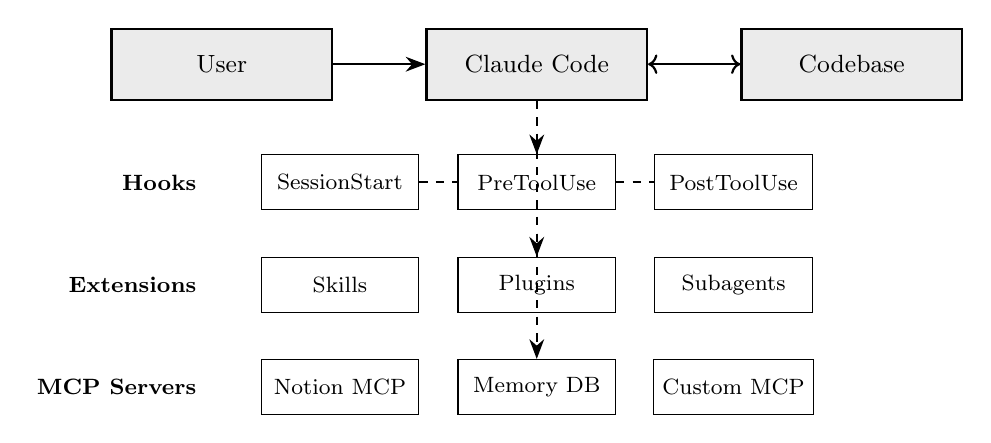
\begin{tikzpicture}[
  box/.style={rectangle, draw, minimum width=2.8cm, minimum height=0.9cm, font=\small, thick},
  smallbox/.style={rectangle, draw, minimum width=2cm, minimum height=0.7cm, font=\footnotesize},
  arr/.style={-{Stealth[length=2.5mm]}, thick},
  every node/.style={align=center}
]
  % Core
  \node[box, fill=black!8] (user) at (0,0) {User};
  \node[box, fill=black!8] (claude) at (4,0) {Claude Code};
  \node[box, fill=black!8] (files) at (8,0) {Codebase};

  \draw[arr] (user) -- (claude);
  \draw[arr, <->] (claude) -- (files);

  % Layer 1: Hooks
  \node[smallbox] (hook1) at (1.5, -1.5) {SessionStart};
  \node[smallbox] (hook2) at (4, -1.5) {PreToolUse};
  \node[smallbox] (hook3) at (6.5, -1.5) {PostToolUse};

  \draw[arr, dashed] (claude) -- (hook2);
  \draw[dashed, thick] (hook1) -- (hook2) -- (hook3);
  \node[font=\footnotesize\bfseries, anchor=east] at (-0.2, -1.5) {Hooks};

  % Layer 2: Skills & Plugins
  \node[smallbox] (sk1) at (1.5, -2.8) {Skills};
  \node[smallbox] (sk2) at (4, -2.8) {Plugins};
  \node[smallbox] (sk3) at (6.5, -2.8) {Subagents};

  \draw[arr, dashed] (claude) -- (sk2);
  \node[font=\footnotesize\bfseries, anchor=east] at (-0.2, -2.8) {Extensions};

  % Layer 3: External
  \node[smallbox] (mcp1) at (1.5, -4.1) {Notion MCP};
  \node[smallbox] (mcp2) at (4, -4.1) {Memory DB};
  \node[smallbox] (mcp3) at (6.5, -4.1) {Custom MCP};

  \draw[arr, dashed] (claude) -- (mcp2);
  \node[font=\footnotesize\bfseries, anchor=east] at (-0.2, -4.1) {MCP Servers};

\end{tikzpicture}

\vspace{1.5cm}

{\large 29 repositories $\cdot$ 8 domains $\cdot$ 1,500+ skills surveyed}

\vspace{0.3cm}

{\normalsize 6 key sources deep-absorbed $\cdot$ 3 rounds adversarial review}

\vspace{2cm}

\textcolor{gray}{\small Yggdra $\cdot$ Personal Knowledge System}

\textcolor{gray}{\small March 2026}

\end{center}
\newpage

% ============================================================
% TABLE OF CONTENTS
% ============================================================
\tableofcontents
\newpage

% ============================================================
% ABSTRACT
% ============================================================
\section{Abstract}

Claude Code is Anthropic's official command-line interface for working with Claude directly in the terminal or an IDE. Rather than using a browser chat, you type in your terminal and Claude reads files, edits code, runs commands, and works across entire projects. Since its launch, a full ecosystem has emerged around it---skills, plugins, hooks, memory systems, workflow frameworks, and visual tools---created both by Anthropic and by the community.

This report surveys that ecosystem as of March 2026. 29 repositories and sources have been reviewed across 8 domains. Each repository is evaluated individually: what it does, when it fits, what caveats to consider, and whether better alternatives exist. The report provides deep technical explanations of core concepts (context windows, hooks, MCP, subagents, context rot), a gap analysis against an existing production system (Yggdra), and a concrete implementation plan.

\textbf{Key findings:}
\begin{itemize}
  \item The ecosystem is dominated by a small number of high-quality repositories (ECC, GSD, claude-mem) that have established patterns now imitated by hundreds of smaller projects.
  \item \textbf{Progressive disclosure}---retrieving information in layers rather than all at once---is the single most impactful innovation for token efficiency.
  \item \textbf{Hooks} (automatic triggers on events) are more reliable than skills (instructions Claude chooses to follow) for critical workflows.
  \item Most repositories solve one of three problems: memory persistence, workflow structure, or token optimization. Very few address all three.
  \item The official Anthropic plugins are conservative but reliable. Community tools are more ambitious but carry dependency and maintenance risks.
\end{itemize}

\newpage

% ============================================================
% METHOD
% ============================================================
\section{Method}

\subsection{Research Process}

The report was produced in five phases:

\begin{description}[leftmargin=0pt, style=nextline]
  \item[\textbf{Phase 1: Broad survey}]
  Systematic review of GitHub repositories via \texttt{gh} CLI and WebFetch. Sources found through: Anthropic official repos, community awesome-lists, Hacker News discussions, YouTube. All raw data saved in \texttt{research-dump-claude-code-ecosystem.md} (363 lines). Grouped into 8 domains.

  \item[\textbf{Phase 2: Deep absorption}]
  5 parallel agents absorbed 6 key sources. Each agent had specific extraction goals: read README, source code, config files, templates. Extract schemas, hooks, workflows, patterns. 1 agent stalled and was manually replaced (ISS-001).

  \item[\textbf{Phase 3: Evaluation}]
  Each tool classified using the ThoughtWorks Technology Radar model with 4 criteria: maturity (stars, community activity, maintenance cadence), relevance to Yggdra, cost/risk (license terms, dependencies, token overhead), and overlap with existing tools.

  \item[\textbf{Phase 4: Adversarial review (3 rounds)}]
  Red team attacks recommendations and finds weaknesses. Blue team defends or concedes. Neutral judge implements changes. 9 corrections from this process.

  \item[\textbf{Phase 5: Self-critique (3 rounds)}]
  Structural critique (missing sections?), content critique (are claims substantiated?), usability critique (can a reader act on this?). 8 additional fixes.
\end{description}

\subsection{Limitations}

\begin{itemize}
  \item \textbf{Star counts} indicate popularity, not validated quality.
  \item \textbf{Token savings claims} (e.g.\ claude-mem's ``$\sim$10x'') are from the sources' own benchmarks, not independently verified.
  \item \textbf{Snapshot in time:} All data is from March 8, 2026. The ecosystem evolves rapidly.
  \item \textbf{Selection bias:} Only English-language, GitHub-hosted repos are included.
\end{itemize}

\newpage

% ============================================================
% CORE CONCEPTS
% ============================================================
\section{Core Concepts --- Deep Dive}

\subsection{Claude Code}

Claude Code is a terminal program. You start it with the command \texttt{claude} and then write in natural language---``find all TODO comments in src/'' or ``add a login page.'' Claude reads files, edits code, runs tests, and navigates the entire project. It differs from a browser chat because Claude has direct access to the filesystem and terminal.

Claude Code can also run inside an IDE (e.g.\ VS Code) as a sidebar panel, so you see code and Claude's work side by side. All skills, hooks, and MCP servers work identically in both modes.

\textbf{What Claude Code is not:} It is not an autonomous agent that runs indefinitely. It responds to prompts, uses tools, and stops. Autonomy must be built on top---via hooks, cron jobs, or external orchestration.

\subsection{The Context Window}
\label{sec:context-window}

The context window is the total amount of information Claude can ``see'' at once. As of March 2026, it is 200,000 tokens ($\approx$150,000 words). This sounds like a lot, but it fills quickly:

\begin{center}
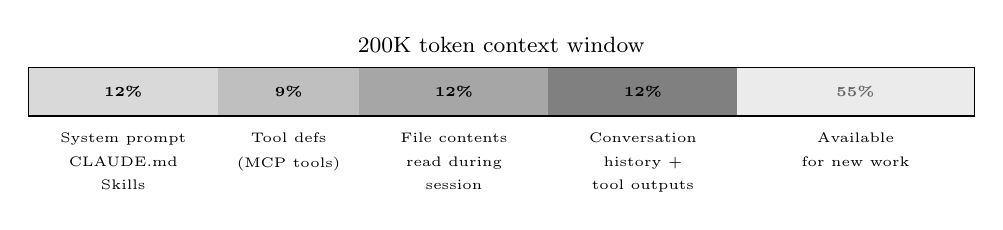
\begin{tikzpicture}[
  bar/.style={rectangle, draw, thick, minimum height=0.6cm, anchor=west},
  label/.style={font=\footnotesize, anchor=east}
]
  % Total bar
  \draw[thick] (0,0) rectangle (12, 0.6);
  \node[font=\footnotesize] at (6, 0.9) {200K token context window};

  % Segments
  \fill[black!15] (0,0) rectangle (2.4, 0.6);
  \fill[black!25] (2.4,0) rectangle (4.2, 0.6);
  \fill[black!35] (4.2,0) rectangle (6.6, 0.6);
  \fill[black!50] (6.6,0) rectangle (9.0, 0.6);
  \fill[black!8] (9.0,0) rectangle (12, 0.6);

  % Labels below
  \node[font=\tiny, anchor=north] at (1.2, -0.1) {System prompt};
  \node[font=\tiny, anchor=north] at (1.2, -0.4) {CLAUDE.md};
  \node[font=\tiny, anchor=north] at (1.2, -0.7) {Skills};

  \node[font=\tiny, anchor=north] at (3.3, -0.1) {Tool defs};
  \node[font=\tiny, anchor=north] at (3.3, -0.4) {(MCP tools)};

  \node[font=\tiny, anchor=north] at (5.4, -0.1) {File contents};
  \node[font=\tiny, anchor=north] at (5.4, -0.4) {read during};
  \node[font=\tiny, anchor=north] at (5.4, -0.7) {session};

  \node[font=\tiny, anchor=north] at (7.8, -0.1) {Conversation};
  \node[font=\tiny, anchor=north] at (7.8, -0.4) {history +};
  \node[font=\tiny, anchor=north] at (7.8, -0.7) {tool outputs};

  \node[font=\tiny, anchor=north] at (10.5, -0.1) {Available};
  \node[font=\tiny, anchor=north] at (10.5, -0.4) {for new work};

  % Percentage labels
  \node[font=\tiny\bfseries] at (1.2, 0.3) {12\%};
  \node[font=\tiny\bfseries] at (3.3, 0.3) {9\%};
  \node[font=\tiny\bfseries] at (5.4, 0.3) {12\%};
  \node[font=\tiny\bfseries] at (7.8, 0.3) {12\%};
  \node[font=\tiny\bfseries, text=black!60] at (10.5, 0.3) {55\%};
\end{tikzpicture}
\end{center}

These percentages are approximate and shift during a session. The key insight: \textbf{before Claude does any real work, 30--50\% of the window may already be consumed} by system prompt, tool definitions, and loaded files. With too many MCP servers, the available space shrinks dramatically---ECC reports that 200K can effectively become $\sim$70K with excessive tooling.

\textbf{Token costs (Opus 4.6):} Input tokens cost \$15 per million; output tokens cost \$75 per million. A session consuming 200K tokens costs approximately \$3. Token efficiency is therefore both a quality concern (more room for useful content) and a financial one.

\subsection{Context Rot}

Context rot is the degradation of Claude's output quality over the course of a long session. It happens because:

\begin{enumerate}
  \item The context window fills with file contents, tool outputs, error messages, and conversation history.
  \item When the window approaches capacity, Claude Code \textbf{automatically compresses} the older portion of the conversation. This is called ``compaction.''
  \item Compaction is lossy---details from earlier in the session are summarized or dropped entirely.
  \item Claude may ``forget'' decisions made earlier, repeat mistakes, or lose track of the overall plan.
\end{enumerate}

\textbf{Symptoms of context rot:}
\begin{itemize}
  \item Claude asks questions that were already answered
  \item Code changes conflict with earlier changes in the same session
  \item Claude loses track of which files it has already modified
  \item Output quality drops noticeably compared to the start of the session
\end{itemize}

\textbf{Mitigation strategies} (explored in detail in later sections):
\begin{itemize}
  \item \textbf{Fresh context per task} (GSD pattern): spawn a new subagent for each subtask
  \item \textbf{Context monitor hooks}: warn at 35\% remaining, halt at 25\%
  \item \textbf{Strategic compaction}: manually compact at logical breakpoints
  \item \textbf{State files}: save progress to disk so it survives compaction
\end{itemize}

\subsection{Skills}
\label{sec:skills}

A \textbf{skill} is a reusable instruction for Claude Code, stored as a markdown file in the \texttt{.claude/skills/} directory. When Claude encounters a task matching the skill's description, it follows the instructions in the file.

\textbf{Example:} A skill called ``commit-message'' contains rules for how commit messages should be formatted in a specific project. Every time Claude makes a commit, it follows those rules automatically.

Skills can also be \textbf{user-invocable}---started manually with a slash command like \texttt{/commit} or \texttt{/review}. They can accept arguments (\texttt{/deploy staging}), run shell commands as preprocessing, and spawn subagents that work in isolation.

\textbf{Key skill properties:}
\begin{description}
  \item[\texttt{context: fork}] The skill runs in an isolated subagent with its own context. Results return to the main conversation. Useful for heavy tasks that shouldn't pollute the main context.
  \item[\texttt{allowed-tools}] Restricts which tools the skill may use. A read-only skill can be limited to Read and Grep.
  \item[\texttt{model}] Overrides the model. A cheap scan skill can use Haiku; an architecture skill can require Opus.
  \item[\texttt{!\`{}command\`{}}] Shell commands that run \textbf{before} the skill is sent to Claude. Output replaces the placeholder. This is preprocessing, not runtime execution.
  \item[\texttt{\$ARGUMENTS}] Replaced with the user's input. \texttt{\$ARGUMENTS[0]} for positional arguments.
  \item[Budget] Skills may occupy at most 2\% of the context window ($\sim$16,000 characters as fallback). Override with \texttt{SLASH\_COMMAND\_TOOL\_CHAR\_BUDGET}.
\end{description}

\subsection{Hooks}
\label{sec:hooks}

Hooks are automatic actions that execute when specific events occur in Claude Code. They are shell scripts (bash, Python, Node) executed by the system---not by Claude itself. This distinction matters: Claude ``chooses'' whether to follow a skill's instructions (and sometimes doesn't), but hooks fire with 100\% reliability because they are hard triggers.

% Hook lifecycle flow diagram
\begin{center}
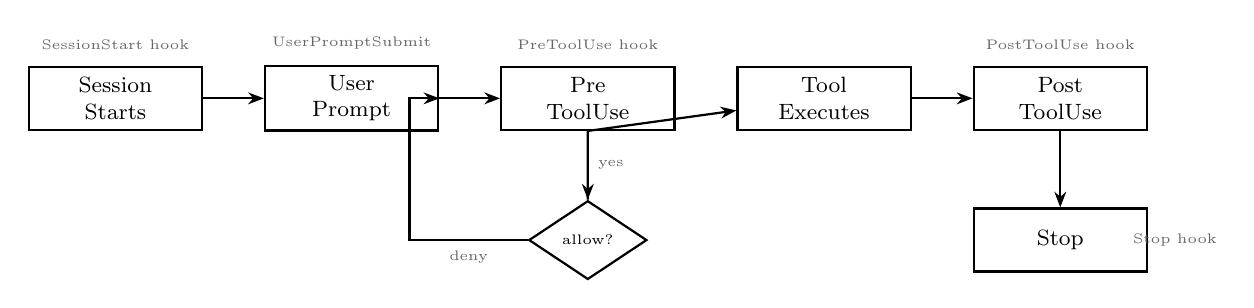
\begin{tikzpicture}[
  box/.style={rectangle, draw, thick, minimum width=2.2cm, minimum height=0.8cm, font=\footnotesize, align=center},
  decision/.style={diamond, draw, thick, minimum width=1.5cm, minimum height=1cm, font=\tiny, align=center, inner sep=1pt},
  arr/.style={-{Stealth[length=2mm]}, thick},
  note/.style={font=\tiny, text=black!60}
]
  \node[box] (start) at (0,0) {Session\\Starts};
  \node[box] (prompt) at (3,0) {User\\Prompt};
  \node[box] (pretool) at (6,0) {Pre\\ToolUse};
  \node[decision] (allow) at (6,-1.8) {allow?};
  \node[box] (tool) at (9,0) {Tool\\Executes};
  \node[box] (posttool) at (12,0) {Post\\ToolUse};
  \node[box] (stop) at (12, -1.8) {Stop};

  \draw[arr] (start) -- (prompt);
  \draw[arr] (prompt) -- (pretool);
  \draw[arr] (pretool) -- (allow);
  \draw[arr] (allow) -- node[note, right] {yes} (allow |- tool.south) -- (tool);
  \draw[arr] (allow.west) -- node[note, below] {deny} ++(-1.5,0) |- (prompt);
  \draw[arr] (tool) -- (posttool);
  \draw[arr] (posttool) -- (stop);

  % Hook annotations
  \node[note, above] at (0, 0.5) {SessionStart hook};
  \node[note, above] at (3, 0.5) {UserPromptSubmit};
  \node[note, above] at (6, 0.5) {PreToolUse hook};
  \node[note, above] at (12, 0.5) {PostToolUse hook};
  \node[note, right] at (12.8, -1.8) {Stop hook};
\end{tikzpicture}
\end{center}

\textbf{Hook output format:} Hooks communicate with Claude Code via JSON on stdout:

\begin{lstlisting}
{
  "hookSpecificOutput": {
    "hookEventName": "PreToolUse",
    "permissionDecision": "deny",
    "permissionDecisionReason": "Edits on main blocked."
  }
}
\end{lstlisting}

There are \textbf{17 hook events} in total. The most important ones:

\begin{description}
  \item[SessionStart] Fires when a session starts. Used to load context, previous state, or inject instructions. Matchers: \texttt{startup}, \texttt{resume}, \texttt{clear}, \texttt{compact}.
  \item[UserPromptSubmit] Fires when the user sends a message. Can \textbf{modify} the message before Claude sees it. Used to add context or redirect.
  \item[PreToolUse] Fires before Claude uses a tool (Edit, Bash, Write, etc.). Can \textbf{block} the tool. Used for safety---e.g.\ preventing edits on the main branch. Matchers: tool name regex.
  \item[PostToolUse] Fires after a tool succeeds. Used for auto-formatting, auto-testing, or data collection. Non-blocking.
  \item[PreCompact] Fires before Claude compresses its context. Used to save important state before it is lost.
  \item[Stop] Fires when Claude finishes its response. Used for checkpoints.
  \item[SubagentStart / SubagentStop] Fires when subagents spawn or finish. Used for logging and rate-limiting.
\end{description}

\textbf{Hook priority order:} Managed policy $>$ \texttt{\textasciitilde/.claude/settings.json} $>$ \texttt{.claude/settings.json} $>$ \texttt{.claude/settings.local.json} $>$ Plugin hooks $>$ Skill frontmatter hooks.

\subsection{MCP (Model Context Protocol)}
\label{sec:mcp}

MCP is a standard for giving Claude Code access to external systems. An \textbf{MCP server} is a program that exposes tools which Claude can call. For example, a Notion MCP server runs locally and gives Claude tools like ``search pages,'' ``create page,'' and ``update page.''

MCP servers are configured in \texttt{.mcp.json} (project-level) or \texttt{.mcp.json.local} (machine-specific):

\begin{lstlisting}
{
  "mcpServers": {
    "notion": {
      "command": "npx",
      "args": ["-y", "@notionhq/notion-mcp-server"],
      "env": {"OPENAPI_MCP_HEADERS": "..."}
    }
  }
}
\end{lstlisting}

\textbf{Critical insight:} Every tool an MCP server exposes consumes tokens in the context window just by existing (the tool definition must be present for Claude to know it is available). This means \textbf{fewer MCP servers = more space for actual work}. ECC recommends a maximum of 10 MCP servers and 80 active tools. Beyond that, the effective context window shrinks dramatically.

The alternative to always-loaded MCP servers is \textbf{CLI-wrapped skills}: shell commands wrapped in a skill that only loads when invoked. This uses zero tokens when idle.

\subsection{Subagents}
\label{sec:subagents}

A subagent is a separate Claude instance spawned by the main conversation. It gets its own context (typically a fresh 200K window) and works in isolation on a subtask. When finished, it returns the result to the main conversation.

% Subagent architecture mindmap
\begin{center}
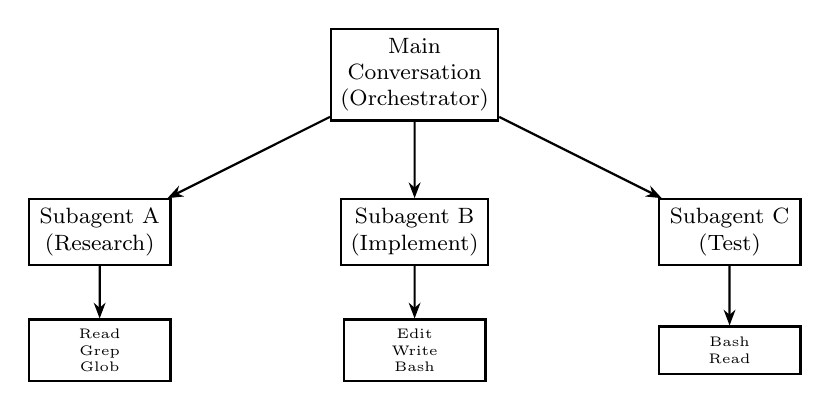
\begin{tikzpicture}[
  level 1/.style={sibling distance=4cm, level distance=2cm},
  level 2/.style={sibling distance=2.2cm, level distance=1.5cm},
  every node/.style={rectangle, draw, thick, font=\footnotesize, minimum width=1.8cm, minimum height=0.6cm, align=center},
  edge from parent/.style={draw, thick, -{Stealth[length=2mm]}},
]
  \node {Main\\Conversation\\(Orchestrator)}
    child { node {Subagent A\\(Research)}
      child { node[font=\tiny] {Read\\Grep\\Glob} }
    }
    child { node {Subagent B\\(Implement)}
      child { node[font=\tiny] {Edit\\Write\\Bash} }
    }
    child { node {Subagent C\\(Test)}
      child { node[font=\tiny] {Bash\\Read} }
    };
\end{tikzpicture}
\end{center}

\textbf{Trade-offs:}
\begin{itemize}
  \item Each spawn costs $\sim$200K tokens ($\approx$\$0.60--1.00) before the subagent does any work.
  \item The subagent has no access to the main conversation's history---it starts fresh.
  \item Multiple subagents can run in parallel, which is powerful for independent tasks.
  \item Coordination between subagents requires explicit design (shared files, state on disk).
\end{itemize}

In skills, use \texttt{context: fork} to spawn a subagent. In conversation, use the Agent or Task tool.

\subsection{Token Economics}

A summary of costs relevant to ecosystem tool choices:

\begin{tabularx}{\textwidth}{l X r}
\toprule
\textbf{Item} & \textbf{Description} & \textbf{Approx.\ cost} \\
\midrule
Opus 4.6 input & Per 1M tokens & \$15 \\
Opus 4.6 output & Per 1M tokens & \$75 \\
Sonnet 4.6 input & Per 1M tokens & \$3 \\
Sonnet 4.6 output & Per 1M tokens & \$15 \\
Haiku 4.5 input & Per 1M tokens & \$0.80 \\
Haiku 4.5 output & Per 1M tokens & \$4 \\
\midrule
Typical Opus session & 200K tokens mixed & $\sim$\$3--5 \\
GSD subagent spawn & 200K fresh context each & $\sim$\$0.60--1 \\
5 parallel subagents & GSD wave execution & $\sim$\$3--5 \\
ECC hooks overhead & Per tool call (standard) & $\sim$500--2K tokens \\
\bottomrule
\end{tabularx}

\textbf{Key principle:} Every optimization that reduces token consumption---progressive disclosure, CLI-wrapped skills, strategic model selection---pays for itself both in cost savings and in better output quality (more room for useful context).

\newpage

% ============================================================
% REPOSITORY CATALOG
% ============================================================
\section{Repository Catalog --- Official Anthropic}

Each repository is evaluated on: what it does, when it fits, caveats, and whether better alternatives exist.

\subsection{anthropics/skills (86.9k stars)}

\textbf{What it is:} The official skills standard definition and reference implementation. This is the canonical source for how skills work: frontmatter syntax, lifecycle, discovery rules, and the \texttt{agentskills.io} specification.

\textbf{What it contains:} Documentation, schema definitions, and reference skills. Not a collection of ready-to-use skills---rather, the specification that all other skill repos follow.

\textbf{When it fits:} Always. If you build or install any skills, this is the authoritative reference.

\textbf{Caveats:} The specification evolves. Features like \texttt{context: fork} and \texttt{hooks} in frontmatter are relatively new. Pin to a version or check the changelog before relying on bleeding-edge features.

\textbf{Alternatives:} None. This is the standard.

\subsection{anthropics/claude-code (75.1k stars)}

\textbf{What it is:} The Claude Code CLI itself, plus \textbf{13 official plugins}. The repo contains both the core tool and first-party extensions.

\textbf{The 13 plugins in detail:}

\begin{description}
  \item[hookify] Creates hooks via natural language. Say ``block edits on main'' and it generates the correct hook configuration. Useful because writing hook JSON manually is error-prone.

  \item[security-guidance] PreToolUse hook that checks for 9 security anti-patterns before Claude executes:
  \begin{enumerate}
    \item SQL injection in Bash commands
    \item Hardcoded credentials/API keys in code
    \item Unsafe deserialization
    \item Command injection via user input
    \item XSS in HTML/JS output
    \item Path traversal in file operations
    \item Insecure HTTP (vs HTTPS)
    \item Over-privileged permissions
    \item Sensitive data in logs/output
  \end{enumerate}

  \item[commit-commands] Adds \texttt{/commit} and \texttt{/commit-push-pr}. The former creates well-formatted conventional commits. The latter goes the full distance: commit, push, create Pull Request with description.

  \item[feature-dev] 7-phase development workflow: discover $\rightarrow$ plan $\rightarrow$ implement $\rightarrow$ test $\rightarrow$ review $\rightarrow$ commit $\rightarrow$ PR. Spawns multiple subagents at each phase.

  \item[code-review] 5 parallel review agents analyze code from different angles (correctness, performance, security, readability, testing).

  \item[pr-review-toolkit] Structured PR review with checklist. Less ambitious than code-review but more practical for daily use.

  \item[plugin-dev] Helps build new plugins. Meta-tool.

  \item[ralph-wiggum] Humorous response format. Not practically useful.

  \item[frontend-design] Frontend-focused skill for UI development. Understands CSS frameworks, component libraries, responsive design.

  \item[explanatory-output-style] Forces Claude to explain its reasoning. Good for learning; adds overhead for production work.

  \item[learning-output-style] Teaching-friendly output with step-by-step explanations.

  \item[agent-sdk-dev] Help for building with the Agent SDK.

  \item[claude-opus-4-5-migration] Migration helper for Opus 4.5 code patterns.
\end{description}

\textbf{When it fits:} The three ``must-install'' plugins are hookify, security-guidance, and commit-commands. They have zero risk (official source), low overhead, and solve common needs. The others are situational.

\textbf{Caveats:} feature-dev and code-review spawn multiple subagents and can be expensive (\$5--10 per invocation). Use them for important work, not routine changes.

\subsection{anthropics/claude-cookbooks (34.4k stars)}

\textbf{What it is:} Practical recipes from Anthropic. Step-by-step tutorials for common patterns.

\textbf{Key recipes:}
\begin{itemize}
  \item \textbf{RAG (Retrieval-Augmented Generation):} How to combine search in your own data with Claude. Directly relevant for any Qdrant-based setup.
  \item \textbf{Tool use:} Designing custom tools and integrations.
  \item \textbf{PDF \& Vision:} Working with documents and images.
  \item \textbf{Sub-agents:} Patterns for multi-agent workflows.
  \item \textbf{SQL \& Data:} Structured data manipulation.
\end{itemize}

\textbf{When it fits:} When building new integrations or learning Claude's tool use patterns. Reference material, not installable.

\textbf{Caveats:} Some recipes may lag behind the latest API. Check dates.

\textbf{Alternatives:} claude-quickstarts for more complete starter projects.

\subsection{anthropics/courses (19.2k stars)}

\textbf{What it is:} Anthropic Academy---13 free courses with certificates. Course materials (Jupyter notebooks, slides) are in this repo.

\textbf{Most relevant courses:}
\begin{description}
  \item[Introduction to Agent Skills] Foundational understanding of skills. Prerequisite for everything else.
  \item[Claude Code in Action (1 session)] Practical walkthrough of Claude Code features: hooks, skills, multi-file editing, subagents.
  \item[MCP Advanced Topics] Depth on Model Context Protocol: custom servers, tool design, performance optimization.
  \item[Tool Use \& Function Calling] How Claude interacts with tools. Important for designing good skills and hooks.
  \item[Prompt Engineering for Developers] Generally useful for writing better skills and CLAUDE.md instructions.
\end{description}

\textbf{When it fits:} For onboarding. Recommended order: Agent Skills $\rightarrow$ Claude Code in Action $\rightarrow$ MCP Advanced.

\textbf{Caveats:} Courses are introductory. They teach concepts, not production patterns.

\subsection{anthropics/claude-quickstarts (15.1k stars)}

\textbf{What it is:} Starter projects from Anthropic.

\textbf{Key starters:}
\begin{description}
  \item[Autonomous Coding Agent] Two-agent pattern: a planner and an executor. Planner breaks down the task; executor implements each step. Similar principle to GSD but simpler.
  \item[Computer Use Demo] Claude controls a computer via screenshots + clicks/keystrokes.
\end{description}

\textbf{When it fits:} When building custom agent pipelines from scratch. The Autonomous Coding Agent pattern is a good starting point before adopting GSD.

\textbf{Caveats:} These are demos, not production-ready frameworks.

\subsection{anthropics/claude-code-action (6.1k stars)}

\textbf{What it is:} GitHub Actions integration for Claude Code. Run Claude as part of CI/CD pipelines.

\textbf{When it fits:} When you want automated code review on PRs, periodic documentation updates, or dependency audits---all powered by Claude. See claude-code-showcase for concrete workflow examples.

\textbf{Caveats:} Each GitHub Actions run consumes Claude API tokens. Set max-turns and timeout limits to control costs. A monthly docs-sync run with 30 turns can cost \$5--10.

\subsection{anthropics/claude-agent-sdk-python (5.2k stars)}

\textbf{What it is:} Python SDK for building custom agents that use Claude as their ``brain.'' The agent runs as a Python process and calls Claude's API for decisions.

\textbf{When it fits:} When building automation scripts that need Claude's reasoning---e.g.\ a research pipeline that reads papers, extracts findings, and organizes them. Or a monitoring agent that reads logs and takes action.

\textbf{Caveats:} Requires Python programming. The SDK handles conversation management and tool use, but you design the agent's architecture. Not a no-code solution.

\textbf{Alternatives:} For simpler automation, Claude Code + hooks + cron may be sufficient.

\newpage

% ============================================================
% COMMUNITY: SKILLS & MEMORY
% ============================================================
\section{Repository Catalog --- Community Skills \& Memory}

\subsection{affaan-m/everything-claude-code [ECC] (65.8k stars)}

\textbf{What it is:} The largest and most influential community collection. 65 skills, 16 agent configurations, 3 in-depth guides. But ECC's real contribution is not just skills---it is a \textbf{philosophy} for using Claude Code effectively.

\textbf{Core principles:}
\begin{itemize}
  \item \textbf{Token optimization:} Keep MCP servers minimal. Replace always-loaded MCP with CLI-wrapped skills that only consume tokens when invoked.
  \item \textbf{Model selection:} Use Haiku for exploration/docs. Sonnet for 90\% of coding. Opus only for bugs, 5+ file changes, architecture, or security.
  \item \textbf{Dynamic context injection:} \texttt{claude --system-prompt "\$(cat memory.md)"} injects context with higher authority than CLAUDE.md.
  \item \textbf{Verification metrics:} pass@k (at least 1 of k attempts succeeds) vs pass\textasciicircum k (all k must succeed). At k=1: 70\%. At k=3: pass@k=91\% but pass\textasciicircum k=34\%. Takeaway: let Claude retry---success rate improves dramatically.
  \item \textbf{Skill audit:} \texttt{/skill-stocktake}---Quick Scan or Full Stocktake. Verdicts: Keep, Improve, Update, Retire, Merge.
\end{itemize}

\textbf{Continuous Learning v2.1} is ECC's most innovative feature. It uses atomic ``instincts'' with confidence scoring:

\begin{lstlisting}
id: prefer-functional-style
trigger: "when writing new functions"
confidence: 0.7    # 0.3=tentative, 0.5=moderate,
                    # 0.7=strong, 0.9=near-certain
domain: "code-style"
scope: project      # or 'global'
project_id: "a1b2c3d4"  # hash of git remote URL
\end{lstlisting}

The observation pipeline fires on \textbf{every} PreToolUse and PostToolUse (hooks = reliable). It scrubs secrets via regex, auto-archives at 10MB, purges after 30 days, and scopes observations to projects via git remote URL hash. When the same instinct appears in 2+ projects with average confidence $\geq$0.8, it auto-promotes to global scope.

\textbf{3 hook profiles:}

\begin{tabularx}{\textwidth}{X c c c}
\toprule
\textbf{Hook} & \textbf{minimal} & \textbf{standard} & \textbf{strict} \\
\midrule
Session start/end, cost tracking & \checkmark & \checkmark & \checkmark \\
Quality gates, auto-format, TS check & --- & \checkmark & \checkmark \\
Continuous learning observe & --- & \checkmark & \checkmark \\
tmux + git push reminders & --- & --- & \checkmark \\
\bottomrule
\end{tabularx}

\textbf{When it fits:} Everyone. Start with the minimal profile (session persistence + cost tracking) and graduate upward.

\textbf{Caveats:} The standard and strict profiles add overhead per tool call (500--2,000 tokens for observation + quality gates). Monitor latency. The continuous learning pipeline requires understanding the observation format before it delivers value.

\textbf{Alternatives:} For just the learning aspect, Self-Improving Agent (alirezarezvani) is simpler. For just the hooks, claude-code-showcase has comparable quality gates.

\subsection{thedotmack/claude-mem (33.4k stars)}

\textbf{What it is:} The most sophisticated memory system in the community. Solves the fundamental problem: Claude forgets everything between sessions.

\textbf{Progressive disclosure---the core innovation:}

Traditional retrieval fetches all content at once. Search for ``transport routes,'' get 20 results, and Claude receives the full content of all 20---typically 10--20K tokens. Most results are irrelevant, but the tokens are spent.

Progressive disclosure solves this with \textbf{3 layers}:

\begin{center}
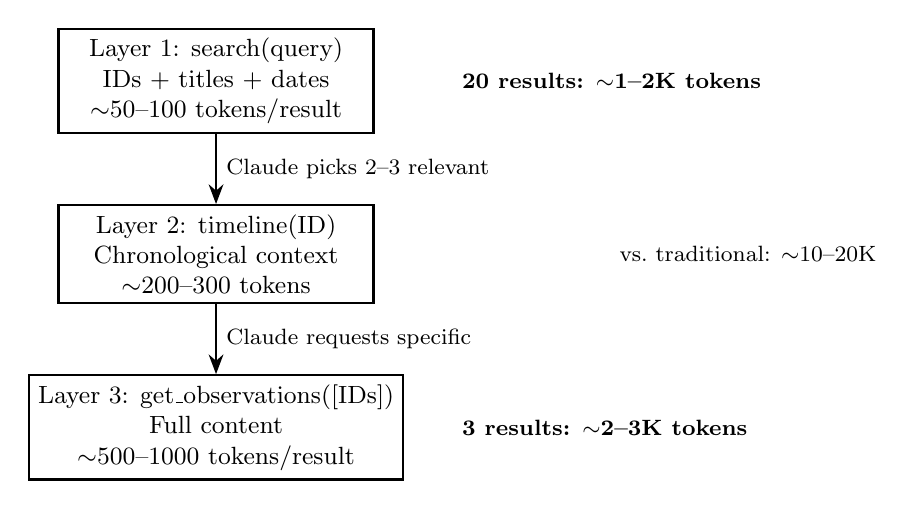
\begin{tikzpicture}[
  box/.style={rectangle, draw, thick, minimum width=4cm, minimum height=1cm, font=\small, align=center},
  arr/.style={-{Stealth[length=2.5mm]}, thick},
]
  \node[box] (l1) at (0, 0) {Layer 1: search(query)\\IDs + titles + dates\\$\sim$50--100 tokens/result};
  \node[box] (l2) at (0, -2.2) {Layer 2: timeline(ID)\\Chronological context\\$\sim$200--300 tokens};
  \node[box] (l3) at (0, -4.4) {Layer 3: get\_observations([IDs])\\Full content\\$\sim$500--1000 tokens/result};

  \draw[arr] (l1) -- node[right, font=\footnotesize] {Claude picks 2--3 relevant} (l2);
  \draw[arr] (l2) -- node[right, font=\footnotesize] {Claude requests specific} (l3);

  \node[font=\footnotesize, anchor=west] at (3, 0) {\textbf{20 results: $\sim$1--2K tokens}};
  \node[font=\footnotesize, anchor=west] at (3, -4.4) {\textbf{3 results: $\sim$2--3K tokens}};
  \node[font=\footnotesize, anchor=west] at (5, -2.2) {vs.\ traditional: $\sim$10--20K};
\end{tikzpicture}
\end{center}

\textbf{Architecture:} SQLite is the source of truth (7 tables, FTS5 for keyword search, WAL mode, 256MB mmap). Chroma is a secondary index for semantic search. Each field in an observation (narrative, fact\_0, fact\_1, etc.) becomes a separate Chroma document---\textbf{granular per-field embedding} that matches on individual facts rather than whole observations.

\textbf{Token savings on two levels:}
\begin{enumerate}
  \item \textbf{AI compression:} Raw tool output ($\sim$5,000 tokens) is compressed into structured observations with title, subtitle, narrative, facts ($\sim$500--1,000 tokens).
  \item \textbf{Progressive disclosure:} Even compressed content is only fetched when relevant.
\end{enumerate}

\textbf{When it fits:} When memory across sessions is critical and you need production-grade retrieval. Best for users who work across many sessions on the same project and frequently need to recall past decisions, discussions, or code changes.

\textbf{Caveats:}
\begin{itemize}
  \item \textbf{AGPL-3.0 license:} Source code must be published if the system is exposed over a network (AGPL \S 13). For private local use (MCP over stdio), risk is low but non-zero.
  \item \textbf{Bun runtime required:} If your stack is Python/bash, Bun is a new dependency to maintain.
  \item \textbf{ragtime/ subdirectory} uses PolyForm Noncommercial 1.0.0---prohibits all commercial use.
  \item The ``$\sim$10x token savings'' claim is from claude-mem's own benchmarks, not independently verified.
\end{itemize}

\textbf{Alternatives:} Build a 3-layer retrieval system yourself against an existing vector database (e.g.\ Qdrant). Simpler, no license issues, but requires implementation work.

\subsection{alirezarezvani/claude-skills (2.3k stars)}

\textbf{What it is:} 160+ skills, with the standout being the \textbf{Self-Improving Agent}---a system that lets Claude learn from its own patterns over time.

\textbf{Self-Improving Agent commands:}
\begin{description}
  \item[/si:review] Scans MEMORY.md for recurring patterns. Identifies which observations keep appearing.
  \item[/si:promote] Graduates confirmed patterns from MEMORY.md (temporary) to CLAUDE.md (permanent). This is the key action: important knowledge that would otherwise be lost when MEMORY.md overflows is promoted to a durable instruction.
  \item[/si:extract] Converts patterns into standalone skills that can be reused across projects.
  \item[/si:status] Memory capacity dashboard.
\end{description}

\textbf{When it fits:} When MEMORY.md fills up with repeated observations that should be permanent instructions. The promotion pipeline solves a real gap: knowledge that gets rediscovered every session instead of being codified once.

\textbf{Caveats:} The promotion process is aggressive---review what it promotes to CLAUDE.md. A wrong pattern codified as a permanent instruction is worse than no instruction.

\textbf{Alternatives:} ECC Continuous Learning v2.1 is more sophisticated (confidence scoring, project scoping) but heavier to set up.

\subsection{Jeffallan/claude-skills (5.6k stars)}

\textbf{What it is:} 66 skills focused on development workflow. The standout is \texttt{/common-ground}.

\textbf{/common-ground:} Surfaces Claude's assumptions about the project. When starting work, Claude may silently assume things about the tech stack, coding conventions, or project goals. This skill forces Claude to explicitly state its assumptions so you can correct them before work begins.

Also includes Jira and Confluence workflow integrations for enterprise teams.

\textbf{When it fits:} At the start of a new project or when onboarding Claude to an unfamiliar codebase. The assumption-surfacing pattern prevents wasted work from wrong assumptions.

\textbf{Caveats:} Jira/Confluence integrations assume enterprise tooling. The standalone skills are more broadly useful.

\textbf{Alternatives:} You can achieve similar assumption-surfacing by adding a rule to CLAUDE.md: ``Before starting any new task, state your assumptions and wait for confirmation.''

\subsection{sickn33/antigravity-awesome-skills (21.6k stars)}

\textbf{What it is:} The largest skills collection---1,232 skills across all categories.

\textbf{When it fits:} As a browsing catalog. When you need a skill for a specific niche (e.g.\ Kubernetes deployment, Terraform plans, GraphQL schema generation), search this repo first.

\textbf{Caveats:} Quality varies enormously. Many skills are trivial wrappers. No curation or quality guarantee. Always read a skill's source before installing it---some may contain unsafe patterns.

\textbf{Alternatives:} For curated, high-quality skills, start with ECC or the official plugins. Use Antigravity Awesome only when you need something specific that doesn't exist elsewhere.

\subsection{VoltAgent/awesome-claude-code-subagents}

\textbf{What it is:} Collection of 127+ subagent configurations across 10 domains, each with isolated context windows.

\textbf{When it fits:} When designing multi-agent architectures. The value is in the design patterns, not the specific configurations (which need adaptation to your stack).

\textbf{Caveats:} Many subagent configs are generic. The interesting ones are domain-specific (e.g.\ security-focused, data-pipeline-focused). Copy the pattern, adapt the specifics.

\textbf{Alternatives:} NicholasSpisak's 9 personas (see Workflow section) are more focused and opinionated.

\subsection{makenotion/claude-code-notion-plugin}

\textbf{What it is:} Official plugin from Notion for Claude Code. Adds 4 skills and 10 slash commands on top of the built-in Notion MCP.

\textbf{Skills:}
\begin{description}
  \item[Knowledge Capture] Auto-saves important findings to Notion during a session.
  \item[Meeting Intelligence] Structures meeting notes and action items.
  \item[Research Documentation] Organizes research findings in databases.
  \item[Spec to Implementation] Converts Notion specifications into code.
\end{description}

\textbf{When it fits:} When Notion is your primary organizational tool and you want deeper integration than the basic MCP provides.

\textbf{Caveats:} Known Cowork-mode bug (Issue \#18680): tools disappear after first prompt. Workaround: restart session. Notion MCP cannot create views (Kanban, Calendar)---views must be created manually in Notion's UI.

\textbf{Alternatives:} The built-in Notion MCP handles 80\% of use cases. This plugin adds the remaining 20\%.

\subsection{YouMind-OpenLab/nano-banana-pro-prompts}

\textbf{What it is:} 10,000+ curated prompts for Google Gemini's image generation model (Gemini 3 Pro Image / Nano Banana Pro).

\textbf{When it fits:} When generating visual content---diagrams, infographics, illustrations, concept art---using Gemini's native image generation. The prompts are structured with subject, medium, style, lighting, composition, and palette.

\textbf{Caveats:} Gemini-specific. These prompts do not transfer well to other image models (DALL-E, Midjourney). Requires Google Gemini API access.

\textbf{Alternatives:} For Claude-native visual generation, use Mermaid (diagrams) or the diagrams Python library (infrastructure). For general image generation, use whatever model you have API access to.

\subsection{tfriedel/claude-office-skills}

\textbf{What it is:} Skills for working with Microsoft Office formats: PPTX, DOCX, XLSX, PDF.

\textbf{When it fits:} When Claude needs to generate or modify Office documents. Useful for automated report generation, presentation building, or spreadsheet manipulation.

\textbf{Caveats:} Heavy dependency chain (python-pptx, python-docx, openpyxl). The skills assume specific Python libraries are installed. Quality of generated documents varies---complex formatting is difficult to get right programmatically.

\textbf{Alternatives:} For PDF: LaTeX (which this report uses). For presentations: Mermaid diagrams exported to slides. For spreadsheets: direct CSV/JSON manipulation is often simpler.

\subsection{mksglu/context-mode (2.9k stars)}

\textbf{What it is:} A tool that compresses context to reduce token usage. It pre-processes files and conversation history to be more token-efficient before sending to Claude.

\textbf{When it fits:} When working with large codebases where many files need to be in context simultaneously. It compresses boilerplate and repetitive code patterns.

\textbf{Caveats:} Cannot intercept MCP tools---only works with direct file operations. Less relevant for setups that already use selective file loading.

\textbf{Alternatives:} Progressive disclosure (claude-mem) solves the same problem more fundamentally. Strategic model selection (Haiku for exploration, Opus for critical work) is a simpler approach.

\newpage

% ============================================================
% WORKFLOW & ARCHITECTURE
% ============================================================
\section{Repository Catalog --- Workflow \& Architecture}

\subsection{gsd-build/get-shit-done [GSD] (26.1k stars)}

\textbf{What it is:} The most comprehensive workflow framework for Claude Code. Solves context rot by decomposing large tasks into small, independently-executable plans with fresh context per task.

% GSD workflow process flow
\begin{center}
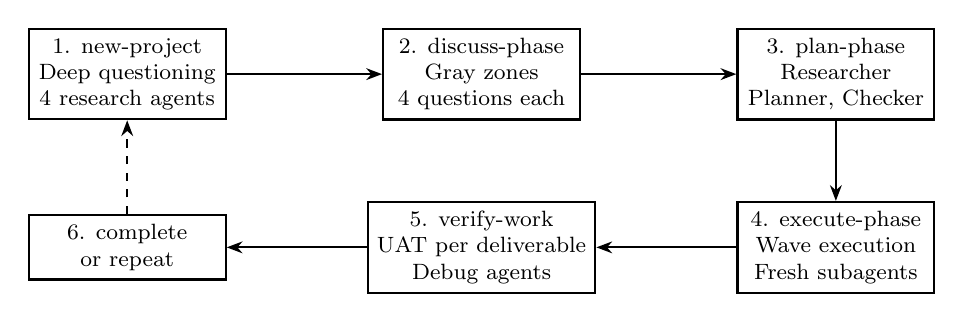
\begin{tikzpicture}[
  box/.style={rectangle, draw, thick, minimum width=2.5cm, minimum height=0.8cm, font=\footnotesize, align=center},
  arr/.style={-{Stealth[length=2mm]}, thick},
]
  \node[box] (new) at (0, 0) {1. new-project\\Deep questioning\\4 research agents};
  \node[box] (disc) at (4.5, 0) {2. discuss-phase\\Gray zones\\4 questions each};
  \node[box] (plan) at (9, 0) {3. plan-phase\\Researcher\\Planner, Checker};

  \node[box] (exec) at (9, -2.2) {4. execute-phase\\Wave execution\\Fresh subagents};
  \node[box] (ver) at (4.5, -2.2) {5. verify-work\\UAT per deliverable\\Debug agents};
  \node[box] (done) at (0, -2.2) {6. complete\\or repeat};

  \draw[arr] (new) -- (disc);
  \draw[arr] (disc) -- (plan);
  \draw[arr] (plan) -- (exec);
  \draw[arr] (exec) -- (ver);
  \draw[arr] (ver) -- (done);
  \draw[arr, dashed] (done) -- (new);
\end{tikzpicture}
\end{center}

\textbf{STATE.md} (<150 lines): A slim pointer file containing Project Reference, Current Position (phase/status/ASCII progress bar), Performance Metrics (velocity, trend), Accumulated Context (decisions, blockers), and Session Continuity (timestamp, resume path).

\textbf{Wave execution:} Plans have dependencies defined in PLAN.md frontmatter:

\begin{lstlisting}
---
phase: 01-auth
plan: 03
wave: 2
depends_on: [plan-01, plan-02]
files_modified: [src/auth/login.ts]
autonomous: true
---
\end{lstlisting}

Wave number: \texttt{wave = max(dependency\_waves) + 1}. Within a wave: parallel. Between waves: sequential. Spot-check after each wave. Config: \texttt{max\_concurrent\_agents: 3}.

\textbf{Fresh context per task:} Each plan is executed by a spawned subagent with 200K clean context. The subagent loads: PLAN.md, config.json, STATE.md (paths only), CLAUDE.md, skills. It does \textbf{not} load: session history, full project context, decision logs. The orchestrator stays at 10--15\% context utilization.

\textbf{4 deviation rules:}
\begin{enumerate}
  \item Bug $\rightarrow$ auto-fix
  \item Missing Critical (validation, auth) $\rightarrow$ auto-add
  \item Blocking (dependencies, imports) $\rightarrow$ auto-fix
  \item Architectural $\rightarrow$ \textbf{STOP} and ask user
\end{enumerate}

\textbf{When it fits:} Large features that span multiple files and take more than one session. Projects where context rot has caused visible quality degradation. Teams where multiple people need to understand the work plan.

\textbf{Caveats:} Heavy. The full GSD workflow (new-project $\rightarrow$ discuss $\rightarrow$ plan $\rightarrow$ execute $\rightarrow$ verify) is overkill for small tasks. The sweet spot is adopting \textbf{principles} without installing the framework: fresh context per task (already possible via Task tool), deviation rules (add to CLAUDE.md), context monitor (a simple hook).

\textbf{Alternatives:} claude-quickstarts' Autonomous Coding Agent for a simpler two-agent pattern. Or just use Task/Agent tools directly with discipline.

\subsection{ChrisWiles/claude-code-showcase (5.5k stars)}

\textbf{What it is:} Practical hooks, quality gates, and CI/CD workflows for Claude Code. Where GSD provides the strategy, showcase provides the tactical implementation.

\textbf{Skill Evaluation Hooks---3 layers:}

\begin{enumerate}
  \item \textbf{skill-eval.sh}---Bash wrapper on UserPromptSubmit. Pipes stdin to JavaScript.
  \item \textbf{skill-eval.js} ($\sim$300 lines)---7 signal types with scoring: Keywords (weight 2), Keyword patterns (3), Path patterns (4), Directory mapping (5), Intent patterns (4), Content patterns (3), Context patterns (2). Minimum confidence 3, top 5 results, exclude patterns.
  \item \textbf{skill-rules.json}---19 skills defined with triggers, excludePatterns, priority, relatedSkills.
\end{enumerate}

This system automatically selects the right skill based on the user's prompt. It is essentially a local, rule-based routing layer.

\textbf{Quality Gate Hooks:}
\begin{itemize}
  \item \textbf{PreToolUse (Edit|Write):} Branch protection---blocks edits on main.
  \item \textbf{PostToolUse (Edit|Write):} Auto-format (Prettier), auto-install (npm), auto-test, type-check (tsc --noEmit). All non-blocking---they provide feedback but don't stop work.
\end{itemize}

\textbf{4 GitHub Actions workflows:}

\begin{tabularx}{\textwidth}{l l X}
\toprule
\textbf{Workflow} & \textbf{Cadence} & \textbf{Function} \\
\midrule
Docs Sync & Monthly & 30 max-turns, 60 min timeout \\
Code Quality & Weekly (Sunday) & 3 random src/ dirs, 35 turns, 45 min \\
Dependency Audit & Biweekly & npm outdated + audit, reverts on test failure \\
PR Code Review & On PR creation & Automatic review \\
\bottomrule
\end{tabularx}

\textbf{When it fits:} TypeScript/JavaScript projects with established CI/CD. The quality gates are directly usable. The skill evaluation pattern is worth studying even if you don't use JavaScript.

\textbf{Caveats:} JavaScript/Node-centric. The PostToolUse hooks assume npm, Prettier, and TypeScript. Adapt for other stacks.

\textbf{Alternatives:} For branch protection alone, a 5-line bash hook is sufficient (see Implementation Plan). For auto-formatting, integrate your stack's formatter (Black for Python, rustfmt for Rust, etc.).

\subsection{NicholasSpisak/claude-code-subagents}

\textbf{What it is:} 9 specialized subagent personas, each with a defined focus area and priority hierarchy.

\begin{tabularx}{\textwidth}{l X}
\toprule
\textbf{Persona} & \textbf{Priority order} \\
\midrule
backend-reliability & Reliability $>$ Security $>$ Performance $>$ Readability \\
frontend-ux & UX $>$ Accessibility $>$ Performance $>$ Consistency \\
systems-architect & Scalability $>$ Maintainability $>$ Security $>$ Performance \\
security-threat & Security $>$ Compliance $>$ Integrity $>$ Availability \\
performance-optimizer & Latency $>$ Throughput $>$ Resource usage $>$ Scalability \\
code-analyzer & Readability $>$ Correctness $>$ Consistency $>$ Efficiency \\
refactoring-expert & Modularity $>$ Testability $>$ Readability $>$ DRY \\
qa-test & Coverage $>$ Reliability $>$ Maintainability $>$ Speed \\
technical-mentor & Understanding $>$ Best practice $>$ Context $>$ Progression \\
\bottomrule
\end{tabularx}

\textbf{Design principle:} Specialization over generalization. Each agent knows a lot about its domain and little about everything else. Combining 3--4 agents provides broader coverage than a single generalist.

\textbf{When it fits:} Code review and architectural decisions where multiple perspectives matter. Run 3 specialized agents in parallel for a comprehensive review.

\textbf{Caveats:} The specific context budgets (50\%/70\%/85\%) mentioned in some discussions could not be verified against the actual repository (ISS-002).

\textbf{Alternatives:} The official code-review plugin provides 5 parallel review agents. VoltAgent has 127+ configurations. Both are less opinionated about priority hierarchies.

\subsection{shanraisshan/claude-code-best-practice}

\textbf{What it is:} A curated collection of best practices for Claude Code usage, gathered from community experience.

\textbf{When it fits:} Quick reference for common patterns and anti-patterns. Good onboarding material.

\textbf{Caveats:} Community-maintained, not official. Practices may not reflect the latest Claude Code features.

\textbf{Alternatives:} ECC's guides are more comprehensive. Official docs are authoritative.

\subsection{teambrilliant/claude-research-plan-implement [RPI]}

\textbf{What it is:} Research-Plan-Implement workflow. A lighter alternative to GSD focused on three phases: research the codebase, plan the changes, implement them.

\textbf{When it fits:} Medium-complexity tasks where GSD's 6-phase workflow is too heavy but you still want structured planning. Good for feature additions that touch 3--5 files.

\textbf{Caveats:} Less mature than GSD. Fewer safeguards against context rot.

\textbf{Alternatives:} GSD for large tasks. Direct Claude Code for small tasks. RPI fills the middle ground.

\subsection{dontriskit/awesome-ai-system-prompts}

\textbf{What it is:} Collection of system prompts from various AI tools, including Claude Code's internal system prompt.

\textbf{When it fits:} Understanding how Claude Code works internally. The system prompt reveals Claude's built-in behaviors, restrictions, and patterns. Useful for debugging unexpected behavior.

\textbf{Caveats:} System prompts change with updates. What you see may not match the current version.

\textbf{Alternatives:} Official documentation for current behavior.

\subsection{lbjlaq/Antigravity-Manager}

\textbf{What it is:} A proxy that routes AI requests through free model providers, potentially giving access to Opus 4.6 without API costs.

\textbf{When it fits:} If API budget is a hard constraint and you need to experiment with expensive models.

\textbf{Caveats:} CC-BY-NC-SA license (non-commercial). Free model providers may have rate limits, quality issues, or disappear without notice. Not suitable for production or sensitive work.

\textbf{Alternatives:} Anthropic's own API with Sonnet (significantly cheaper than Opus) for most work. Budget management via cost monitoring.

\subsection{alibaba/page-agent}

\textbf{What it is:} AI-powered DOM manipulation tool from Alibaba. Claude can interact with web pages by understanding and modifying their structure.

\textbf{When it fits:} Web scraping, automated testing, or web application development where Claude needs to understand page structure.

\textbf{Caveats:} Enterprise-oriented. Heavy dependency on Alibaba's ecosystem. Not well-suited for personal use.

\textbf{Alternatives:} Playwright or Puppeteer for web automation. Claude's built-in Computer Use for visual web interaction.

\newpage

% ============================================================
% VISUAL TOOLS
% ============================================================
\section{Repository Catalog --- Visual Tools}

\subsection{mermaid-js/mermaid (86.5k stars)}

\textbf{What it is:} Converts text-based descriptions into SVG diagrams. The most widely adopted diagramming tool in the developer ecosystem.

\textbf{Supported diagram types:} Flowcharts, sequence diagrams, Gantt charts, class diagrams, state diagrams, entity-relationship, Git graphs, C4 architecture diagrams, mindmaps, timelines.

\textbf{Example:}
\begin{lstlisting}
graph TD
    A[User] --> B[Claude Code]
    B --> C[Hooks]
    B --> D[Skills]
    B --> E[MCP Servers]
    C --> F[save_checkpoint.py]
    D --> G[/commit]
    E --> H[Notion]
\end{lstlisting}

\textbf{When it fits:} Always. Mermaid renders natively in GitHub READMEs, PR descriptions, and Issues. Diagrams are versionable (plain text). Claude generates Mermaid syntax reliably.

\textbf{Caveats:} Complex diagrams with many nodes become unreadable. Mermaid's layout algorithm has limited manual positioning control. For precise layouts, use TikZ or diagrams.

\textbf{Alternatives:} TikZ for print-quality diagrams (what this report uses). diagrams (Python) for infrastructure-specific diagrams. PlantUML for UML-heavy projects.

\subsection{mingrammer/diagrams (42.1k stars)}

\textbf{What it is:} Python library that generates infrastructure diagrams from code. Instead of drawing, you write Python:

\begin{lstlisting}[language=Python]
from diagrams import Diagram, Cluster
from diagrams.onprem.container import Docker
from diagrams.onprem.network import Nginx

with Diagram("Infrastructure"):
    with Cluster("VPS"):
        nginx = Nginx("Traefik")
        app = Docker("Webapp")
        nginx >> app
\end{lstlisting}

\textbf{Supported providers:} AWS, GCP, Azure, Kubernetes, On-Premises, Generic, C4. Uses Graphviz for rendering.

\textbf{When it fits:} Infrastructure documentation. The code-as-diagram approach means diagrams are versionable, reproducible, and reviewable in PRs. Python-native---fits Python-based stacks.

\textbf{Caveats:} Requires Graphviz (\texttt{apt install graphviz}). Output is PNG or PDF, not interactive SVG. The library's icon set is infrastructure-focused---not suitable for general-purpose diagramming.

\textbf{Alternatives:} Mermaid for quick inline diagrams. TikZ for print-quality output. draw.io for interactive editing.

\subsection{antvis/Infographic (4.6k stars)}

\textbf{What it is:} TypeScript library for declarative infographic generation. 200 built-in templates. AI-optimized---Claude can generate configuration objects directly. Streaming render. SVG output.

\textbf{When it fits:} Generating status reports, data visualizations, or presentation-quality infographics programmatically. The templates give quick results without design expertise.

\textbf{Caveats:} TypeScript dependency (doesn't match Python/bash stacks). Still relatively new (4.6k stars). The ``AI-optimized'' claim means the configuration format is LLM-friendly, not that it uses AI internally.

\textbf{Alternatives:} Mermaid for simple diagrams. Matplotlib/Seaborn for data visualization in Python. Gemini image generation (Nano Banana Pro) for creative visuals.

\subsection{federicodeponte/opendraft (55 stars)}

\textbf{What it is:} A 19-agent pipeline that generates academic research drafts (20,000+ words). Uses CrossRef, OpenAlex, Semantic Scholar, and arXiv for citations. Export to PDF, Word, LaTeX.

\textbf{When it fits:} Academic research projects where you need a structured literature review or research draft with proper citations. Uses the same academic APIs as many research scripts.

\textbf{Caveats:} Very low adoption (55 stars). Unproven at scale. The 19-agent pipeline is computationally expensive. Quality of generated academic text needs verification.

\textbf{Alternatives:} Manual research with \texttt{scripts/research.py} + Claude for writing. LaTeX for formatting. The advantage of OpenDraft is automation; the risk is hallucinated citations.

\subsection{Shubhamsaboo/awesome-llm-apps (100k stars)}

\textbf{What it is:} The largest curated collection of LLM applications. Covers RAG tutorials, knowledge graph RAG, multi-agent systems, and applications across all categories.

\textbf{When it fits:} Inspiration and reference. When building a new LLM-powered feature, search this repo for existing implementations to learn from.

\textbf{Caveats:} Breadth over depth. Most examples are starting points, not production code. Quality varies.

\textbf{Alternatives:} claude-cookbooks for Claude-specific recipes. The Python Agent SDK for Claude-native agent building.

\subsection{openclaw/openclaw}

\textbf{What it is:} A personal AI platform with heartbeat daemon, hybrid search, temporal decay, and auto-save. The most architecturally ambitious personal AI system found in this survey.

\textbf{Key principles worth studying:}
\begin{itemize}
  \item \textbf{Heartbeat daemon:} Runs every 30 minutes (not just daily cron). Checks for pending tasks, triggers proactive actions.
  \item \textbf{Hybrid search:} Vector 70\% + BM25 30\% for retrieval. Combines semantic understanding with keyword precision.
  \item \textbf{Temporal decay:} Newer information scores higher. Prevents stale data from dominating results.
  \item \textbf{Auto-save before compaction:} Saves important knowledge before context compression occurs.
\end{itemize}

\textbf{When it fits:} As a design reference. The principles above are gold. The actual codebase is 430K lines of Node.js---too heavy to install.

\textbf{Caveats:} Estimated operational cost: \$2--5K/month. Node.js stack. Not designed for personal single-user systems.

\textbf{Alternatives:} Steal the principles, build simpler implementations. Heartbeat = cron job. Hybrid search = Qdrant configuration. Temporal decay = query-time score adjustment. Auto-save = PreCompact hook.

\newpage

% ============================================================
% GAP ANALYSIS
% ============================================================
\section{Gap Analysis --- Yggdra vs.\ The Ecosystem}

\subsection{What Yggdra already has (validated by the ecosystem)}

\begin{longtable}{p{3.5cm} p{4.5cm} p{5cm}}
\toprule
\textbf{Yggdra feature} & \textbf{Ecosystem equivalent} & \textbf{Assessment} \\
\midrule
\endhead
\texttt{projects/*/NOW.md} & GSD STATE.md, RPI thoughts/ & \textbf{Validated.} GSD adds performance metrics and ASCII progress bar. \\
\midrule
\texttt{projects/*/CONTEXT.md} & ECC per-project CLAUDE.md, GSD PROJECT.md & \textbf{Validated.} GSD further splits into REQUIREMENTS.md and ROADMAP.md. \\
\midrule
save\_checkpoint + load & ECC session hooks, claude-mem hooks & \textbf{Validated.} ECC adds HTML comment markers for idempotent updates. \\
\midrule
episodes.jsonl & claude-mem observations + session\_summaries & \textbf{Primitive.} claude-mem has 7 tables, FTS5, granular observations with confidence scoring. \\
\midrule
4 hook events used & 17 official events available & \textbf{Partial.} Missing UserPromptSubmit, PostToolUse, SubagentStart/Stop. \\
\midrule
\texttt{ctx} (Qdrant search) & claude-mem 3-layer, ECC search-first & \textbf{Partial.} Missing progressive disclosure and FTS5 keyword search. \\
\midrule
CLAUDE.md <200 lines & Best practice, 2\% skill budget & \textbf{Validated.} \\
\midrule
MEMORY.md & claude-mem SQLite, SI Agent, ECC instincts & \textbf{Partial.} Missing auto-promotion, confidence scoring, project scoping. \\
\midrule
Bash-first approach & ECC: CLI-wrappers $>$ MCP & \textbf{Reinforced.} Yggdra's approach confirmed by community consensus. \\
\bottomrule
\end{longtable}

\subsection{What Yggdra is missing (prioritized)}

\begin{enumerate}
  \item \textbf{Quality gate hooks} (high priority, low complexity)---Branch protection + auto-format.
  \item \textbf{Context monitor hook} (high priority, low complexity)---Warn at 35\%, critical at 25\%.
  \item \textbf{Official plugins} (high priority, zero risk)---hookify, security-guidance, commit-commands.
  \item \textbf{Hybrid search} (high priority, medium complexity)---Qdrant supports BM25 + vector natively. Configuration change, not new code.
  \item \textbf{Progressive disclosure} (high priority, high complexity)---3-layer retrieval. Requires baseline measurement first.
  \item \textbf{Auto-promotion} (medium priority, low complexity)---Self-Improving Agent: MEMORY.md $\rightarrow$ CLAUDE.md.
  \item \textbf{Fresh context per task} (medium priority, low complexity)---Already possible via Task tool.
  \item \textbf{Observation extraction} (medium priority, high complexity)---Raw tool output $\rightarrow$ structured observations.
  \item \textbf{Instinct/confidence scoring} (medium priority)---ECC v2.1 project-scoped instincts.
  \item \textbf{Wave execution} (low priority)---GSD dependency mapping. Overkill for now.
\end{enumerate}

\subsection{What Yggdra does better}

\begin{enumerate}
  \item \textbf{Multi-project isolation.} CONTEXT.md + NOW.md per project. GSD has similar features but operates per-project---Yggdra's model handles many projects simultaneously with a single orchestration layer.

  \item \textbf{Episodic memory via cheap LLM.} \texttt{episodes.jsonl} + Groq distillation. No community solution has automatic session distillation via a cheap LLM (claude-mem uses a full Claude instance as worker).

  \item \textbf{Checkpoint safeguards.} 10-min throttle, 80KB cap, hash-dedup. Protects against duplication and overwhelming state files. Not observed in ECC or claude-mem.

  \item \textbf{Kill conditions.} An explicit anti-pattern in CLAUDE.md: ``No new service/cron without a defined condition for removal.'' Not identified in any evaluated repository.

  \item \textbf{Production-grade vector DB.} Qdrant with 84K vectors and 7 collections. Community uses flat files (ECC) or SQLite + Chroma (claude-mem). Yggdra's vector infrastructure is more mature.
\end{enumerate}

\newpage

% ============================================================
% RECOMMENDATIONS
% ============================================================
\section{Recommendations}

\subsection{Classification summary}

Based on the individual repository evaluations, the following classification emerges:

\textbf{Adopt (use now):} VS Code + Extension, Notion MCP (built-in), Anthropic Academy, official plugins (hookify, security-guidance, commit-commands), quality gate hooks, context monitor hook, Mermaid.

\textbf{Trial (experiment actively):} ECC minimal profile, GSD fresh-context principle, claude-mem progressive disclosure, Self-Improving Agent, Notion Plugin, diagrams (Python), Nano Banana Pro.

\textbf{Assess (watch):} ECC Continuous Learning, AntV Infographic, Antigravity Manager, Context Mode, VoltAgent, skill evaluation hooks, OpenDraft, GitHub Actions workflows, GSD wave execution.

\textbf{Hold (park):} Cursor, Google Antigravity (browser), skill marketplaces, Claude Office Skills, OpenSandbox, LaTeX2AI, benbrastmckie/nvim.

\subsection{Implementation plan}

\textit{Sequenced by dependency and impact. Each step is independent of timing.}

\subsubsection{Step 1: Foundation}

\begin{enumerate}
  \item Install VS Code + Claude Code extension on PC
  \item \texttt{git clone} Yggdra repo
  \item Configure \texttt{--add-dir} to VPS copy or symlink
  \item Verify that CLAUDE.md, hooks, and skills load correctly
\end{enumerate}

\subsubsection{Step 2: Official plugins + hooks}

\begin{enumerate}[resume]
  \item Install hookify, security-guidance, commit-commands
  \item Implement branch protection hook (PreToolUse):
\end{enumerate}

\begin{lstlisting}
# Branch protection - denies edits on main
branch=$(git branch --show-current)
if [ "$branch" = "main" ]; then
  echo '{"hookSpecificOutput":{
    "hookEventName":"PreToolUse",
    "permissionDecision":"deny",
    "permissionDecisionReason":"Create a feature branch first."
  }}'
  exit 2
fi
\end{lstlisting}

\begin{enumerate}[resume]
  \item Implement context monitor hook (PostToolUse)
\end{enumerate}

\subsubsection{Step 3: Community trials}

\begin{enumerate}[resume]
  \item Self-Improving Agent: test \texttt{/si:review} and \texttt{/si:promote}
  \item Nano Banana Pro Prompts
  \item Notion Plugin
  \item \texttt{pip install diagrams \&\& apt install graphviz}
\end{enumerate}

\subsubsection{Step 4: Workflow}

\begin{enumerate}[resume]
  \item Test fresh-context-per-task (via Task tool)
  \item Add deviation rules to CLAUDE.md
  \item Evaluate: does it improve quality vs.\ current workflow?
\end{enumerate}

\subsubsection{Step 5: Memory}

\begin{enumerate}[resume]
  \item Measure baseline token consumption via \texttt{cost\_guardian.py}
  \item Evaluate claude-mem: is AGPL \S 13 + Bun acceptable?
  \item Alternative: prototype 3-layer retrieval against Qdrant
  \item Enable hybrid search in Qdrant (BM25 + vector)
\end{enumerate}

\subsubsection{Ongoing}

\begin{itemize}
  \item Anthropic Academy courses (Agent Skills $\rightarrow$ Claude Code in Action $\rightarrow$ MCP Advanced)
  \item ECC minimal profile (\texttt{ECC\_HOOK\_PROFILE=minimal})
  \item Weekly skill-stocktake
  \item Monthly reassessment of Trial and Assess items
\end{itemize}

\newpage

% ============================================================
% MAINTENANCE & KILL CONDITIONS
% ============================================================
\section{Maintenance \& Kill Conditions}

\subsection{Cadences}

\begin{tabularx}{\textwidth}{l X}
\toprule
\textbf{Cadence} & \textbf{Action} \\
\midrule
Daily & Checkpoint + episodes (existing, automatic) \\
Weekly & \texttt{/skill-stocktake} audit of installed skills \\
Monthly & Reassess: have Assess items matured to Trial? \\
Quarterly & Full report update: new sources, star counts, trends \\
\bottomrule
\end{tabularx}

\subsection{Kill conditions}

Every new tool must have a defined removal condition \textbf{before} installation:

\begin{itemize}
  \item \textbf{ECC:} Remove if hooks add $>$5 sec latency per tool call, or user manually disables them $>$3 times/week.
  \item \textbf{claude-mem:} Remove if AGPL \S 13 is incompatible with setup, or Bun dependency creates maintenance burden $>$1 hour/month.
  \item \textbf{Skill evaluation:} Remove if false-positive rate $>$30\%.
  \item \textbf{Notion Plugin:} Remove if it crashes Cowork-mode or adds $>$5 tools to context.
  \item \textbf{Any trial tool:} Remove if not used in 30 days.
\end{itemize}

\subsection{Cost monitoring}

\textbf{Prerequisite:} Measure baseline token consumption per session via \texttt{cost\_guardian.py} \textbf{before} installing new tools. Without a baseline, you cannot measure the effect of new tooling.

\newpage

% ============================================================
% OPEN QUESTIONS
% ============================================================
\section{Open Questions}

\begin{description}[style=nextline]
  \item[1. AGPL \S 13 evaluation]
  claude-mem's AGPL-3.0 license requires source code disclosure if the system is exposed over a network. For private local use (MCP over stdio), the risk is low but non-zero. The \texttt{ragtime/} subdirectory uses PolyForm Noncommercial 1.0.0---prohibits all commercial use.

  \item[2. Bun dependency]
  claude-mem requires Bun runtime. Adding a new runtime means security updates, version conflicts, and debug overhead.

  \item[3. Progressive disclosure MVP]
  A Qdrant endpoint returning IDs + titles + scores (layer 1). Success criterion: retrieval uses $<$2K tokens for scanning 20 results (vs.\ current $\sim$10--20K).

  \item[4. Token cost monitoring for subagents]
  None of the evaluated repositories have a good solution for measuring real token cost per session including subagent overhead.
\end{description}

% ============================================================
% KNOWN ISSUES
% ============================================================
\section{Known Issues}

\begin{tabularx}{\textwidth}{l X l}
\toprule
\textbf{ID} & \textbf{Description} & \textbf{Status} \\
\midrule
ISS-001 & Agent subprocess stalled during PRD+Skills absorption. Manually replaced with direct WebFetch. Possible cause: rate-limiting or context overflow. & Workaround \\
\midrule
ISS-002 & NicholasSpisak context budgets (50/70/85\%) not verifiable against repository. Data retained with caveat. & Acknowledged \\
\bottomrule
\end{tabularx}

\newpage

% ============================================================
% LINK CATALOG
% ============================================================
\section{Complete Link Catalog}

\textit{Star counts as of March 8, 2026.}

\subsection{Official Anthropic}
\begin{itemize}[leftmargin=1em]
  \item \texttt{anthropics/skills} (86.9k)---Official skills standard
  \item \texttt{anthropics/claude-code} (75.1k)---Claude Code + 13 plugins
  \item \texttt{anthropics/claude-cookbooks} (34.4k)---Practical recipes
  \item \texttt{anthropics/courses} (19.2k)---Anthropic Academy
  \item \texttt{anthropics/claude-quickstarts} (15.1k)---Starter projects
  \item \texttt{anthropics/claude-code-action} (6.1k)---GitHub Actions
  \item \texttt{anthropics/claude-agent-sdk-python} (5.2k)---Python Agent SDK
  \item \url{https://agentskills.io}---Skills standard docs
  \item \url{https://anthropic.skilljar.com/}---Anthropic Academy (13 free courses)
  \item \url{https://code.claude.com/docs/en/skills}---Official skills reference
  \item \url{https://code.claude.com/docs/en/hooks}---Official hooks reference
\end{itemize}

\subsection{Community --- Skills \& Memory}
\begin{itemize}[leftmargin=1em]
  \item \texttt{affaan-m/everything-claude-code} (65.8k)---65 skills, 16 agents, 3 guides
  \item \texttt{thedotmack/claude-mem} (33.4k)---Memory + progressive disclosure
  \item \texttt{sickn33/antigravity-awesome-skills} (21.6k)---1,232 skills
  \item \texttt{Jeffallan/claude-skills} (5.6k)---66 skills, /common-ground
  \item \texttt{ChrisWiles/claude-code-showcase} (5.5k)---Hooks, quality gates
  \item \texttt{mksglu/context-mode} (2.9k)---Context compression
  \item \texttt{alirezarezvani/claude-skills} (2.3k)---Self-Improving Agent
  \item \texttt{VoltAgent/awesome-claude-code-subagents}---127+ subagents
  \item \texttt{makenotion/claude-code-notion-plugin}---Official Notion plugin
  \item \texttt{YouMind-OpenLab/nano-banana-pro-prompts}---10,000+ Gemini prompts
  \item \texttt{tfriedel/claude-office-skills}---PPTX, DOCX, XLSX, PDF
\end{itemize}

\subsection{Workflow \& Architecture}
\begin{itemize}[leftmargin=1em]
  \item \texttt{gsd-build/get-shit-done} (26.1k)---Spec-driven workflow, wave execution
  \item \texttt{shanraisshan/claude-code-best-practice}---Best practices
  \item \texttt{teambrilliant/claude-research-plan-implement}---RPI workflow
  \item \texttt{NicholasSpisak/claude-code-subagents}---9 specialized personas
  \item \texttt{dontriskit/awesome-ai-system-prompts}---System prompt internals
  \item \texttt{lbjlaq/Antigravity-Manager}---AI account proxy
  \item \texttt{alibaba/page-agent}---AI DOM manipulation
  \item \texttt{openclaw/openclaw}---Personal AI platform
\end{itemize}

\subsection{Visual Tools}
\begin{itemize}[leftmargin=1em]
  \item \texttt{mermaid-js/mermaid} (86.5k)---Markdown $\rightarrow$ SVG diagrams
  \item \texttt{mingrammer/diagrams} (42.1k)---Python infrastructure diagrams
  \item \texttt{antvis/Infographic} (4.6k)---AI-optimized infographic generation
  \item \texttt{federicodeponte/opendraft} (55)---19-agent research pipeline
  \item \texttt{Shubhamsaboo/awesome-llm-apps} (100k)---LLM apps collection
\end{itemize}

\subsection{Guides \& Articles}
\begin{itemize}[leftmargin=1em]
  \item How I Use Every Claude Code Feature (blog.sshh.io)
  \item Ultimate Claude Code Setup (Medium)
  \item Claude Code Mobile (happy.engineering)
  \item SkillsBento---\url{https://www.skillsbento.com/}
  \item Skillzwave---\url{https://skillzwave.ai/docs/}
  \item Paks---\url{https://paks.stakpak.dev/}
\end{itemize}

\end{document}
